%%%%%%%%%%%%%%%%%%%%%%%%%%%%%%%%%%%%%%%%%%%%%%%%%%%%%%%%%%%%%%%%%%% 
%                                                                 %
%                            CHAPTER                              %
%                                                                 %
%%%%%%%%%%%%%%%%%%%%%%%%%%%%%%%%%%%%%%%%%%%%%%%%%%%%%%%%%%%%%%%%%%%
\chapter{Resultaten en Evaluatie}
Het aanvalsmodel werd tot hiertoe al volledig beschreven en toegelicht, net als
de dataset die gebruikt wordt om de aanval uit te testen. Dit hoofdstuk
bespreekt hoe de evaluatie wordt aangepakt, wat de bekomen resultaten zijn en
wat ze betekenen.

\section{Evaluatie van de aanval}
Het doel van de aanval is om de locatie te voorspellen waar een gebruiker
effectief vertrekt of aankomt bij het uitvoeren van een sportactiviteit,
ondanks het feit dat deze locatie wordt verborgen door het gebruik van een
\ac{EPZ}. Maar indien we dit zouden uittesten op activiteiten die al cloaking
ondergingen door het platform zouden we de bekomen resultaten niet kunnen
valideren. Daarom zullen we de aanval uittesten en evalueren op publieke
activiteiten die geen \ac{EPZ} bevatten, en deze manueel voorzien van een
\ac{EPZ}. Zo kunnen we de bekomen resultaten vergelijken met een referentie,
namelijk de \textit{grondwaarheid} of de \ac{GT}.

\subsection{De grondwaarheid}\label{sec:groundtruth}
De grondwaarheid van een gebruiker is de effectieve woonplaats, of de plaats
waar deze persoon meestal vanuit vertrekt of aankomt. Dit is de locatie die we
beschouwen als degene waarrond de \ac{EPZ} wordt aangebracht, en die wij ultiem
trachten te achterhalen. We bepalen deze locatie door alle activiteiten van een
gebruiker te overlopen, en de begin- of eindpunten die binnen een straal van 50
meter uit elkaar liggen aan dezelfde cluster toe te voegen volgens het
\ac{DBSCAN}-algoritme. Hassan et al.\ stelden dat 50 meter vergelijkbaar is met
een breedte van een gemiddeld perceel, en dat dit dus een goede benadering
vormt voor de maximale afwijking~\cite{sec18has3:online, Verdonck_2022}. Indien
een cluster bestaat uit 15 punten of meer, dan berekenen we hiervan het
gemiddelde en wordt dit gemiddelde gemapt op de roadgraph. Dit gesnapte punt
stelt dan een grondwaarheid voor van deze gebruiker. Let wel, het kan dat éen
gebruiker meerdere grondwaarheden bevat.

Een tweede kanttekening die we hierbij moeten maken is dat de effectieve begin-
en eindlocaties niet altijd perfect op het wegennetwerk zullen liggen. Een
gebruiker kan bijvoorbeeld starten op een parking of een oprijlaan, wat niet
vervat zit in het netwerk. Wij mappen deze dan achteraf op het straatnetwerk,
maar gedurende de upload berekent het platform in kwestie wel de totale
afgelegde afstand tot het effectieve startpunt. Dit kan dus voor een afwijking
bij de predicties zorgen.~\citeauthor{Dhondt} onderzochten deze afwijking door
een \ac{CDF} te plotten die alle afwijkingen visualiseert, en op zoek te gaan
naar het elleboogpunt~\cite{Dhondt}. Het elbow point is een visueel punt in de
curve waar zich een knik voordoet~\cite{Introduc22:online}. Dit duidt in
theorie de optimale afweging tussen lage afwijking en hoge precisie aan. Zo
bekomen~\citeauthor{Dhondt} een drempelwaarde van 22.95 meter om van een
succesvolle aanval te kunnen spreken. Deze drempelwaarde is toepasselijk voor
92\% van de gebruikers.
\begin{figure}[h]
    \centering
    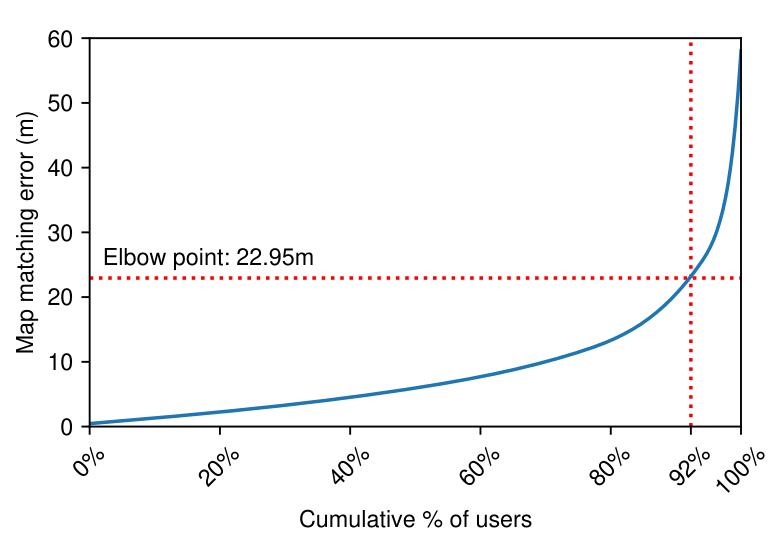
\includegraphics[width=0.8\textwidth]{fig/Afwijkingen&Analyses/OvershootMappingDistance.png}
    \caption{Dhondt et al.\ bepaalt grafisch de trend van de afwijkingen bij het snappen van locaties op het wegennetwerk~\cite{Dhondt}}\label{fig:overshootMappingDistance}
\end{figure}

\subsection{Manueel aanbrengen van een EPZ}\label{sec:zelf_cloaking}
We werken zoals al eerde vermeld met publieke activiteiten die geen \ac{EPZ},
om zo de het evaluatieproces te versimpelen. Maar om de aanval te kunnen
uitvoeren moet we dus nog manueel een \ac{EPZ} aanbrengen. Zo kunnen we een
situatie creëren die de werkelijke situatie benadert, en kunnen we ons
aanvalsmodel uitvoeren. Het is dus wel belangrijk dat de aangebrachte \ac{EPZ}
op een realistische manier wordt aangebracht zodat deze de werkelijkheid
weerspiegelt.

Sectie~\ref{sec:EPZ} bespreekt al uitvoerig het mechanisme van een \ac{EPZ}, en
hoe deze wordt bepaald. Om het even kort te recapituleren, een \ac{EPZ} wordt
bepaald door een centraal punt (de gevoelige locatie), wat een willekeurige
translatie zal ondervinden\footnote{In de context van de beschrijving van
    Hassan et al.\ gebeurd er geen translatie, maar deze thesis gaat wel degelijk
    uit van een model waarbij spatial cloaking op toegepast
    is~\cite{sec18has3:online}.}, en een gekozen straal. Vanaf het getransleerde
punt wordt een cirkel opgezet met de desbetreffende straal. Strava als
fitnessplatform heeft de grootste keuze uit mogelijke stralen, namelijk van 200
meter tot 1600 meter in sprongen van 200 meter. Het doel is om de effectiviteit
van de aanval vast te leggen voor verschillende radiussen, dus zullen we per
gebruiker en per aanvalsmodel een \ac{EPZ} opzetten met alle verschillende
radiussen. Zo kunnen we het effect van de radius zien, maar ook de types aanval
onderling onafhankelijk van de straal vergelijken. We starten dus vanaf de
\ac{GT}. Deze locatie ondervindt dan een willekeurige translatie. De
verschuiving van het punt kan gebeuren in alle richting, en kiezen we dus
willekeurig. De afstand van de translatie kan in principe ook willekeurig
worden gekozen, maar moet wel binnen bepaalde grenzen liggen, namelijk tussen 0
en 70\% van de straal van de \ac{EPZ}. De cirkel kan dan worden opgesteld, met
als middelpunt het getransleerde punt, en de bijhorende straal. Alle punten die
zich binnen deze zone bevinden, zullen worden verwijdert uit de activiteit.
% Figuur: 3 stappen hoe een EPZ wordt opgezet

\subsection{Bootstrapping}
Bij het uittesten van de aanval wordt de aanval niet zomaar een enkele keer
uitgevoerd voor alle activiteiten per gebruiker. Dit zou vertekende resultaten
kunnen geven. Per gebruiker wordt een betrouwbaarheidsinterval berekent via
bootstrapping~\cite{Dhondt, Verdonck_2022}. De set met manueel verhulde
activiteiten wordt beschouwd. Het bootstrapalgoritme kiest hieruit willekeurig
één voor één activiteiten, en plaatst deze in een nieuwe groep totdat deze
nieuwe groep activiteiten even groot is als de originele set van activiteiten.
Let wel, het algoritme kan meerdere malen dezelfde activiteit kiezen, dus met
andere woorden kan de nieuw gemaakte groep duplicaten bevatten en andere
activiteiten helemaal niet bevatten. Dit gebeurt 1000 keer, en er worden dus
1000 verschillende sets gemaakt. Voor elke set zal een voorspelling worden
uitgevoerd. Zo bekomen we een aantal voorspelde locaties, waarvan er een kans
is dat enkele locaties meerdere malen voorspeld worden. Op
Figuur~\ref{fig:bootstrapping} is te zien hoe de distributie eruit ziet op een
kaart~\cite{Verdonck_2022}. Op de figuur zijn de individuele voorspelling
aangeduidt met een blauwe tot paarse kleur, afhankelijk van hoe frequent ze
voorspeld werden (hoe meer naar de paarse of rode kleur ligt, hoe frequenter de
node voorspeld is). Ook zichtbaar zijn de start- en eindpunten, met een
verschillend kleur per \ac{E.G.} De locatie van de grondwaarheid is aangeduid
door de groene marker.

\begin{figure}[h]
    \centering
    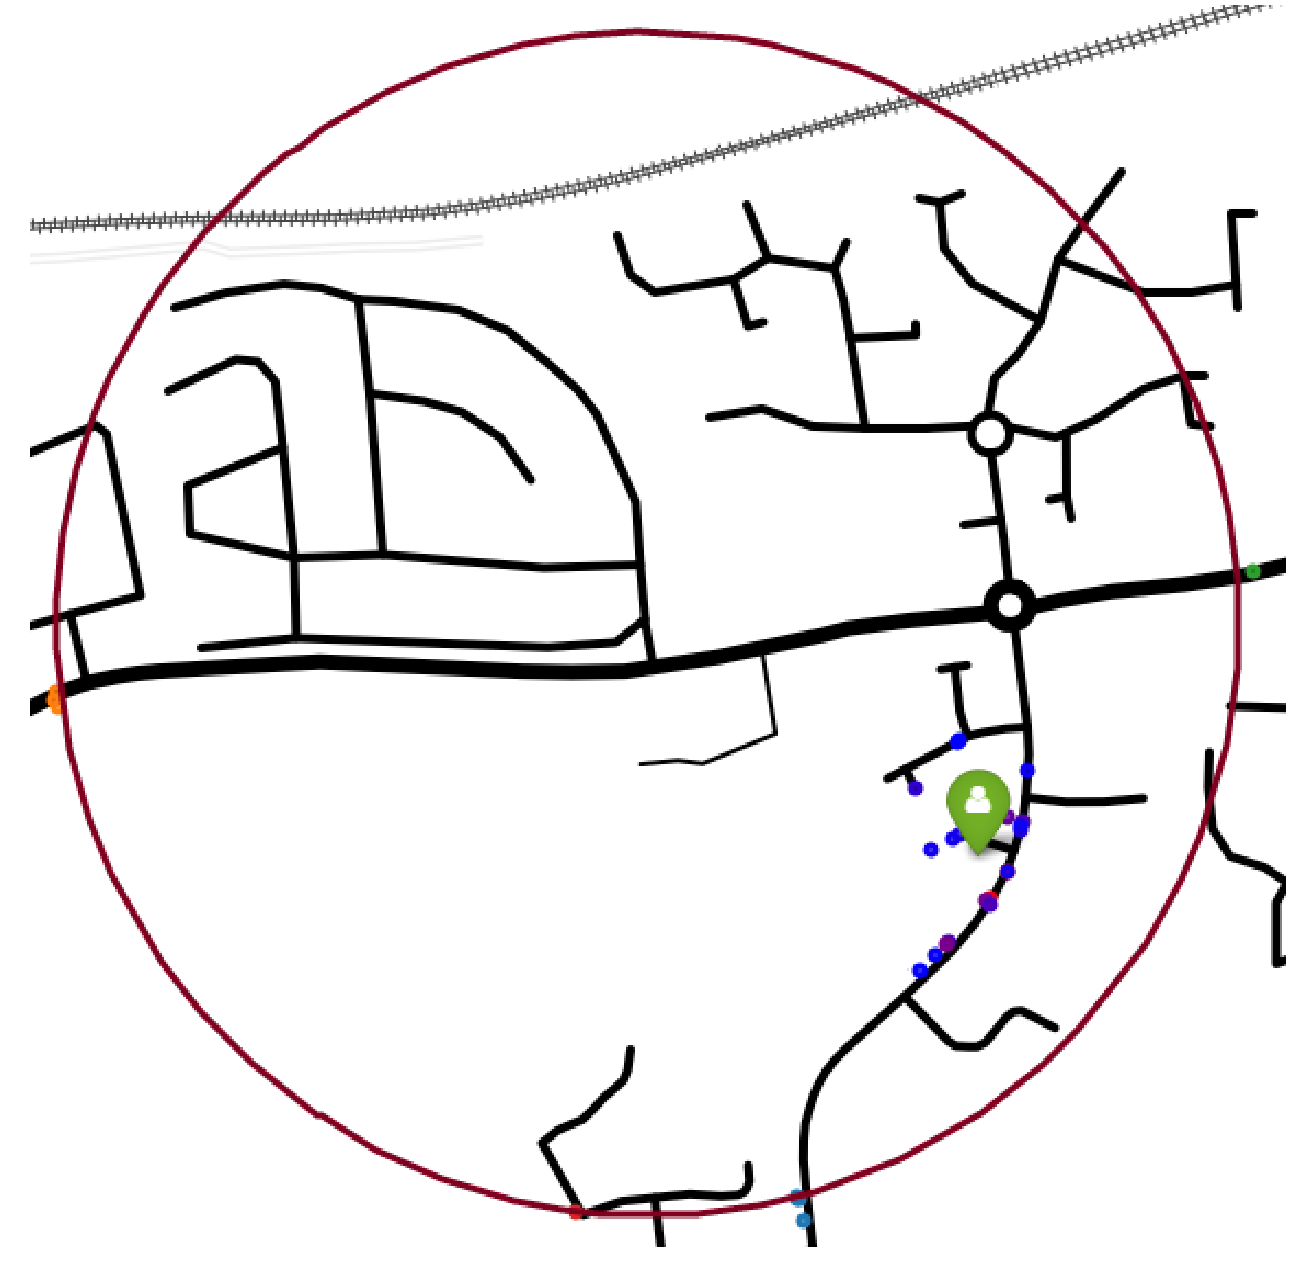
\includegraphics[width=0.6\textwidth]{fig/bootstrapping.png}
    \caption{Voorbeeld van een distributie van voorspellingen bepaald door het bootstrapalgoritme~\cite{Verdonck_2022}}\label{fig:bootstrapping}
\end{figure}

\subsection{Evaluatie metrieken}
Om iets zinnigs te kunnen vertellen over de effectiviteit van de aanval
definiëren we enkele metrieken die we kunnen gebruiken om de aanval te
evalueren. We gebruiken hiervoor de metrieken die ook gebruikt werden in de
studies van~\citeauthor{Dhondt} en~\citeauthor{Verdonck_2022}, om zo onze
resultaten er eenduidig mee te kunnen vergelijken. In totaal gebruiken we acht
verschillende evaluatiemetrieken.

De eerste evaluatie metriek is de \textit{Success Rate}~\cite{Dhondt}. Dit is
het percentage van de uitgevoerde aanvallen waar de gevoelige locatie succesvol
is achterhaald. Rekening houdend met de overshoots die komen met het snappen
van locaties op het wegennetwerk, is een correcte locatie een locatie die zich
binnen een straal van 22.95 meter van de \ac{GT} bevindt. Hoe hoger het
percentage, hoe succesvoller de aanval.

De \textit{Correctness} van een aanval is de som van de Euclidische afstanden
tussen de \ac{GT} en de voorspelde locatie gedeeld door het aantal keer deze
locatie werd voorspeld~\cite{Dhondt, Verdonck_2022}. Dit geeft een indicatie
van de gemiddelde afwijking in afstand van de voorspelde locaties ten opzichte
van de \ac{GT}. Hoe lager deze waarde, hoe preciezer de aanval. Let wel, een
succes rate kan hoog zijn, maar de correctheid kan nog steeds hoog zijn. Dit
duidt op een aanval die veel overshoots heeft, maar waar de correcte locatie
zich wel binnen de straal van 22.95 meter bevindt. De probabiliteitsdistributie
wordt gegeven door $\widehat{\operatorname{Pr}}(v \mid a)$, waarbij $v$ de
beschermde locaties voor activiteit $a$ zijn in
Vergelijking~\ref{eq:correctness}.
\begin{equation}
    \sum_{v \in V} \widehat{\operatorname{Pr}}(v \mid a) \operatorname{dist}\left(v, v_{G T}\right)\label{eq:correctness}
\end{equation}

De \textit{Accuracy} definiëren we als de breedte van het
betrouwbaarheidsinterval~\cite{Dhondt, Verdonck_2022}. Met deze breedte doelen
we op het aantal unieke voorspellingen, het aantal nodes dat precies eenmalig
worden voorspeld. Hoe meer unieke nodes, hoe hoger de accuracy en ook hoe
minder `zeker' onze voorspelling is.

De \textit{Reduction of the k-anonymity set} kwantificeert de de afname in de
set van alle mogelijke eindlocaties voor en na de effectieve predicties van een
aanval~\cite{Dhondt, Verdonck_2022}. De mogelijke eindlocaties voor de aanval
zijn simpelweg alle nodes in de graafvoorstelling, eventueel begrensd door de
\ac{EPZ}. Degene na de aanval zijn alle nodes die effectief voorspelt worden.
De reductie is dus een percentage die het verschil tussen de twee sets
aangeeft. Hoe hoger de reductie, hoe meer nodes verdwijnen uit de set van
mogelijke eindlocaties na de aanval. Dit zegt dus iets over de hoeveelheid
kandidaten het algoritme voorspelt, ten opzichte van hoeveel kandidaten er
mogelijk zijn.
\begin{equation}
    \frac{k-\left|V_{\text {pred }, \text { ext }}\right|}{k}\label{eq:reduction}
\end{equation}

De \textit{Uncertainty Region ($m^2$)} is de som van oppervlaktes van de
unie\footnote{De unie van de oppervlakte van twee cirkels is de som van de twee
    oppervlakten, min één maal het overlappende deel.} van de onzekerheidsregio's
rond de voorspelde nodes~\cite{Dhondt,Verdonck_2022}. De chaining distance, die
in ons geval drie meter aanneemt, veroorzaakt deze onzekerheidsregio's.
Aangezien pas om de drie meter een node bestaat, zal voor elke voorspelde node
een kans bestaan dat deze eigenlijk een punt representeert die ergens in de
zone van drie meter rond deze node ligt. Hoe groter deze waarde, hoe groter de
onzekerheid van de aanval, aangezien dit wijst op weinig overlap. $C_{v_p}$
stelt de cirkel rond een node voor, met straal $d_{\text{chain}}$.
\begin{equation}
    \operatorname{Area}\left(\bigcup_{v_p \in V_{\text {pred }}} C_{v_p}, d_{\text {chain }}\right)\label{eq:uncertainty}
\end{equation}

De \textit{Certainty} definieert de concentratie van de
probabiliteitsdistributie~\cite{Dhondt}. Hoe hoger deze waarde, hoe verder van
elkaar de nodes in de probabiliteitsdistributie liggen.
\begin{equation}
    -\sum_{v \in V} \widehat{\operatorname{Pr}}(v \mid a) \log (\widehat{\operatorname{Pr}}(v \mid a))\label{eq:certainty}
\end{equation}

De \textit{Spatial Certainty} is de certainty, maar in plaats van de
probabiliteit van elke node te beschouwen, gebruiken we de neighboorhood
probabiliteit om zo de densiteit in de buurt van elke node te
beschouwen~\cite{Dhondt}.
\begin{equation}
    -\sum_{v \in V} \widehat{\operatorname{Pr}}(v \mid a) \log \left(\widehat{\operatorname{Pr}_n}(v \mid a)\right)\label{eq:spatial_certainty}
\end{equation}

De laatste evaluatiefactor is de \textit{Degree of
    Anonymity}~\cite{Dhondt,Verdonck_2022}. Dit is de genormaliseerde entropie van
de verwachte distributie. Deze wordt genormaliseerd op basis van de maximale
mogelijke entropie, en wordt bepaald op basis van percentage $p_v$. Dit is een
percentage die aangeeft bij hoeveel percent van de voorspellingen node $p$
voorspelt wordt. Dit zal voor vele nodes gelijk zijn aan 0. De maximale
entropie komt voor indien elke node exactly evenveel voorspelt wordt, en is dus
gelijk aan $\frac{1}{\# nodes}$.
\begin{equation}
    \frac{-\sum_{v \in V} \widehat{\operatorname{Pr}}(v \mid a) \log _2(\widehat{\operatorname{Pr}}(v \mid a))}{H_0(V)}\label{eq:degree_of_anonymity}
\end{equation}

\section{Resultaten}
Nu we alle evaluatiemetrieken besproken hebben, kunnen we overgaan naar de
evaluatie van de geteste scenarios. Elk getest scenario zal afzonderlijk worden
besproken alsook onderling vergeleken worden. De resultaten van de aanvallen
worden weergegeven in tabellen, die telkens voor elke metriek een score
weergeven. Ook draaien we voor (zo goed als) alle beschreven scenario's een
aanval voor enkele radiussen.

Daarnaast worden alle resultaten ook grafisch weergegeven op
Figuur~\ref{fig:attack_comparison}. Dit geeft een mooi globaal overzicht van
alle modellen ten opzichte van elkaar, en maakt de onderlinge verschillen
zichtbaar. Bij de bespreking van de resultaten zullen we dan ook zowel
refereren naar de tabellen als naar de grafieken.

\begin{figure}[h]
    \centering
    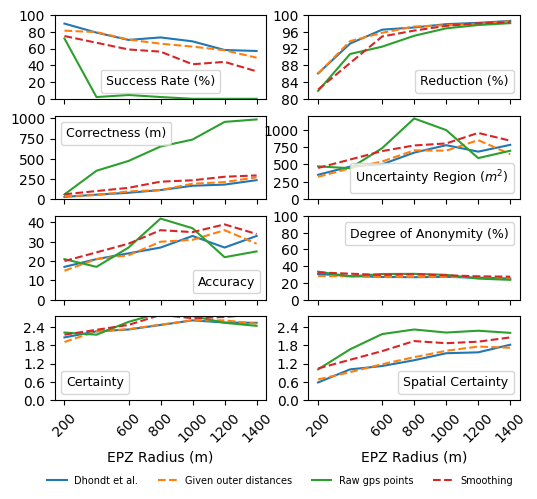
\includegraphics[width=\textwidth]{fig/result_graphs/all_results.png}
    \caption{Vergelijking van de verschillende aanvallen}\label{fig:attack_comparison}
\end{figure}

Over het algemeen is een gelijklopende trend merkbaar over de modellen heen,
bij het veranderen van de \acp{EPZ}. Bij een toenemende radius zakt de
succesratio doordat een grotere radius meer nodes met zich meebrengt. En meer
nodes zorgt voor meer mogelijke verwarring in de \ac{LAD}
regressie~\cite{Verdonck_2022}. Dit brengt ook een grotere degree of anonymity
en uncertainty region met zich mee. Het aantal voorspellingen neemt niet
evenredig toe met het aantal nodes in de graaf naarmate de omvang toeneemt, wat
resulteert in een verhoogde reduction. Als laatste valt ook op dat de
correctness ook stijgt bij een grotere radius. Dit komt door een grotere kans
op schending van één van de gestelde assumpties uit
Sectie~\ref{sec:assumpties}. Deze sectie stelt onder andere dat een gebruiker
het kortste pad moet volgen binnenin de \ac{EPZ}. Echter hoe groter de \ac{EPZ}
van omvang is, hoe groter de kans dat hieraan niet voldaan wordt, en wat zal
resulteren in een hogere correctness.

\subsection{Model volgens Dhondt et al.}
Het eerste model dat we testen is het model van
\citeauthor{Dhondt}~\cite{Dhondt}, Tabel~\ref{tab:aanval_karel} toont de
betreffende resultaten. We gebruiken deze resultaten als referentie voor de
rest van de resultaten. Het model van~\citeauthor{Dhondt} heeft geen
restricties betreffende de beschikbare data, het kan dus alle data gebruiken.
Het is dan ook logisch dat dit resulteert in goeie scores. We zien hier dan ook
een hoge succes rate, die relatief weinig afneemt bij hogere radiussen. De rest
van de statistieken wijzen ook op een goeie aanval, wat naar de verwachtingen
is. Het doel van de andere aanvallen was dan ook deze waardes te benaderen,
maar met alternatieve data.Het aanvalsmodel is geïmplementeerd en uitgevoerd op
ons eigen systeem op de beschikbare fractie van de dataset, wat de lichte
verschillen ten opzichte van de resultaten beschreven in de desbetreffende
paper verklaart.

\begin{table}[h]
    \centering
    \scalebox{0.55}{
        \begin{tabular}{lrrrrrrrr}
            \toprule
            {}         & Success Rate (\%) & Correctness (m) & Accuracy & Reduction (\%) & Uncertainty Region ($m^2$) & Certainty & Spatial Certainty & Degree of Anonymity (\%) \\
            Radius (m) &                   &                 &          &                &                            &           &                   &                          \\
            \midrule
            200        & 89.86             & 28.61           & 17       & 86.06          & 352.08                     & 2.06      & 0.58              & 30.69                    \\
            400        & 79.1              & 56.82           & 21       & 93.21          & 469.76                     & 2.26      & 1.01              & 28.31                    \\
            600        & 70.37             & 79.94           & 24       & 96.52          & 502.42                     & 2.32      & 1.12              & 27.15                    \\
            800        & 73.33             & 113.68          & 27       & 97.05          & 670.53                     & 2.47      & 1.31              & 26.86                    \\
            1000       & 68.64             & 166.74          & 33       & 97.84          & 777.57                     & 2.62      & 1.54              & 27.25                    \\
            1200       & 58.33             & 180.97          & 27       & 98.15          & 684.71                     & 2.55      & 1.57              & 26.25                    \\
            1400       & 57.14             & 235.76          & 33       & 98.61          & 782.30                     & 2.54      & 1.82              & 25.31                    \\
            \bottomrule
        \end{tabular}
    }
    \captionsetup{justification=centering}
    \caption{Aanval volgens het model van Dhondt et al.~\cite{Dhondt}}\label{tab:aanval_karel}
\end{table}

\subsection{Gegeven outer distance}
Het eerste scenario dat we testen is het model waarbij de outer distance
rechtstreeks af te lezen valt uit de data. We bespraken dit geval al
kortstondig in Sectie~\ref{sec:berekeningen}. Dit model komt voor wanneer de
cumulatieve afstanden ter beschikking zijn. Het voordeel dat dit model heeft is
dat er geen \ac{gps}-data nodig is.

Hierbij zien we gelijkaardige trend als bij het model van~\citeauthor{Dhondt},
met op de meeste scores een kleine achteruitgang ten opzichte ervan. Er is
slechts één tussenstap is ten opzichte van het model van~\citeauthor{Dhondt},
namelijk het omreken van snelheid en de tijd tot de totale afstand. Dit
verklaart dan ook meteen de kleine afnames en toenames in de resultaten. Deze
omrekening zal een kleine afwijking met zich meebrengen, waarschijnlijk door
afrondingen en mogelijke additionele berekeningen van Strava bij het berekenen
van de snelheid.

\begin{table}[h]
    \centering
    \scalebox{0.55}{
        \begin{tabular}{lrrrrrrrr}
            \toprule
            {}         & Success Rate (\%) & Correctness (m) & Accuracy & Reduction (\%) & Uncertainty Region ($m^2$) & Certainty & Spatial Certainty & Degree of Anonymity (\%) \\
            Radius (m) &                   &                 &          &                &                            &           &                   &                          \\
            \midrule
            200        & 81.43             & 35.96           & 15       & 86.01          & 322.32                     & 1.91      & 0.68              & 28.33                    \\
            400        & 79.71             & 51.38           & 21       & 93.78          & 445.30                     & 2.26      & 0.92              & 27.80                    \\
            600        & 70.77             & 96.94           & 23       & 95.78          & 542.48                     & 2.33      & 1.18              & 27.34                    \\
            800        & 65.83             & 113.18          & 30       & 97.28          & 703.00                     & 2.48      & 1.41              & 27.38                    \\
            1000       & 62.39             & 191.47          & 31       & 97.60          & 698.69                     & 2.62      & 1.62              & 27.31                    \\
            1200       & 57.98             & 212.06          & 36       & 97.86          & 850.01                     & 2.62      & 1.76              & 27.13                    \\
            1400       & 49.15             & 270.35          & 29       & 98.54          & 648.70                     & 2.51      & 1.72              & 24.90                    \\
            \bottomrule
        \end{tabular}
    }
    \captionsetup{justification=centering}
    \caption{Aanval op basis van gegeven \textit{outer distance}, en snelheid}\label{tab:outerDistance}
\end{table}

\subsection{Ruwe gps-data}
De volgende aanval is deze zonder gegeven cumulatieve afstand, maar ook zonder
smoothing. Dit zorgt ervoor dat de aanvaller de ruwe \ac{gps}-data rechtstreeks
gebruikt voor het berekenen van de outer distance. In dit geval zit zowel de
afwijking die afkomstig is van de snelheidsomrekening, die besproken werd in
het vorige model (waarbij de outer distance gegeven is) alsook de afwijkingen
die afkomstig zijn van de \ac{gps}-data zelf vervat in de resultaten.

De afwijkingen veroorzaakt wegen zoals verwacht relatief sterk door. Zeker bij
grotere radiussen heeft dit een grote impact op de resultaten. Vanaf een radius
van 1000 meter is de success rate zelfs 0\%. Maar ook bij de rest van de
metrieken zien we een aanzienlijk slechtere score een sterke achteruitgang
vertoond bij een hogere \ac{EPZ}-radius. Dit is te wijten aan de grote
afwijkingen die de \ac{gps}-data in zijn geheel met zich mee brengt, zeker bij
grotere radiussen weegt dit sterk door. Hoe groter de af te leggen afstand, in
dit geval de inner distance, hoe groter de fout.
\begin{table}[h]
    \centering
    \scalebox{0.55}{
        \begin{tabular}{lrrrrrrrr}
            \toprule
            {}         & Success Rate (\%) & Correctness (m) & Accuracy & Reduction (\%) & Uncertainty Region ($m^2$) & Certainty & Spatial Certainty & Degree of Anonymity (\%) \\
            Radius (m) &                   &                 &          &                &                            &           &                   &                          \\
            \midrule
            200        & 72.06             & 59.92           & 21       & 81.89          & 473.05                     & 2.22      & 1.01              & 33.43                    \\
            400        & 2.08              & 351.85          & 17       & 90.71          & 446.35                     & 2.15      & 1.67              & 27.80                    \\
            600        & 4.55              & 473.15          & 27       & 92.46          & 734.62                     & 2.57      & 2.17              & 30.67                    \\
            800        & 2.13              & 651.38          & 42       & 95.06          & 1161.95                    & 2.87      & 2.32              & 30.84                    \\
            1000       & 0.00              & 737.93          & 37       & 96.84          & 994.80                     & 2.76      & 2.22              & 29.69                    \\
            1200       & 0.00              & 955.79          & 22       & 97.63          & 592.09                     & 2.54      & 2.28              & 25.16                    \\
            1400       & 0.00              & 986.46          & 25       & 98.08          & 697.50                     & 2.44      & 2.21              & 23.70                    \\
            \bottomrule
        \end{tabular}
    }
    \captionsetup{justification=centering}
    \caption{Aanval op basis van ruwe \ac{gps}-locaties (geen smoothing) en snelheid}\label{tab:noSmoothing}
\end{table}

\subsection{Smoothing}
Het laatste model is gelijkaardig aan het voorgaande, met als verschil dat nu
wel smoothing wordt toegepast op de routes in een poging om de afwijkingen van
de \ac{gps}-data te verminderen. In Sectie~\ref{sec:berekeningen} bescreven we
het mechanisme. Zeker de extremen zullen worden afgevlakt, waardoor de fouten
van een kleinere orde zouden moeten hebben. Dit toont zich ook in de
resultaten. Het gebruikte smoothing-algoritme heeft één parameter die wij
kunnen aanpassen, namelijk de smoothing window. Deze parameter bepaalt hoeveel
punten er per window worden gecombineerd. Het optimale smoothing window wordt
hier bepaald door het uitvoeren van een aantal experimenten, en hiervan de
resultaten met elkaar vergelijken. Deze resultaten zijn terug te vinden in
Bijlage~\ref{ch:smoothing_results} op Tabel~\ref{tab:full_smoothing}. Deze zijn
ietwat wisselvallig, en er is geen duidelijke trend in terug te vinden.
% De hypothese is dat dit komt door de
% factor van willekeur die meespeelt bij het manueel opzetten van de \ac{EPZ}.
% Wanneer afwijkende punten net wel of net niet afgesneden worden door de
% \ac{EPZ}. 
Maar wanneer we zoeken naar het best scorende smoothing window, komen we uit op
een smoothing window van 100. Dit hoge smoothing window wijst wel nog maar eens
op de vele fouten die de \ac{gps}-data bevat.

De success rate toont een relatief kleine verbetering ten opzichte van het
model met de ruwe \ac{gps}-data bij kleine \acp{EPZ}, maar bij grotere
\acp{EPZ} tonen de metrieken veel minder verval. Ook de andere metrieken
vertonen een gelijkaardig patroon, waarbij de afzwakking veel minder sterk is
dan bij het gebruik van ruwe \ac{gps}-punten. Dit toont dat het gebruik van
smoothing zeker een significante toegevoegde waarde heeft. Let wel dit
smoothing window empirisch bepaald en optimaal gekozen voor deze dataset. Voor
een andere dataset kan het optimale window een verschillende waarde aannemen.
\begin{table}[h]
    \centering
    \scalebox{0.5}{
        \begin{tabular}{lrrrrrrrrr}
            \toprule
            {}         &                      & Success Rate (\%) & Correctness (m) & Accuracy & Reduction (\%) & Uncertainty Region ($m^2$) & Certainty & Spatial Certainty & Degree of Anonymity (\%) \\
            Radius (m) & Smoothing Window (n) &                   &                 &          &                &                            &           &                   &                          \\
            \midrule
            200        & 100                  & 75.0              & 61.37           & 20       & 82.22          & 450.15                     & 2.15      & 1.04              & 32.57                    \\
            600        & 100                  & 58.97             & 141.04          & 29       & 94.89          & 692.52                     & 2.47      & 1.61              & 29.51                    \\
            800        & 100                  & 56.34             & 217.13          & 36       & 96.30          & 773.61                     & 2.80      & 1.94              & 30.30                    \\
            1000       & 100                  & 41.27             & 234.27          & 35       & 97.43          & 802.93                     & 2.69      & 1.87              & 29.13                    \\
            1200       & 100                  & 44.12             & 278.00          & 39       & 98.06          & 953.93                     & 2.73      & 1.92              & 27.86                    \\
            1400       & 100                  & 32.81             & 294.24          & 34       & 98.28          & 841.94                     & 2.82      & 2.06              & 27.51                    \\
            \bottomrule
        \end{tabular}
    }
    \captionsetup{justification=centering}
    \caption{Aanval op basis van gesmoothe \ac{gps}-data en snelheid, met een empirisch bepaald optimaal smoothing window $n=100$}\label{tab:optimal_smoothing}
\end{table}

% Figuur: 3 stappen hoe een EPZ wordt opgezet